% !TEX root = ../Dokumentation.tex
\newpage
\subsection{Beladen und Greifer}
\textbf{Änderungen gegenüber PREN1}\\[0.2cm]
Der Greifer wurde fast so umgesetzt wie in PREN1 geplant. Es musste einzig an den Greiferflächen Änderungen vorgenommen werden. Bei den Tests wurde erkannt, dass die Greifer nicht perfekt parallel greifen und das die Haftung nicht ausreichte. Um eine grössere Auflagefläche zu erreichen, sind auf beiden Seiten Bleche angeklebt. Auf die Bleche wurde beidseitig haftendes Klebeband montiert.\\[0.2cm]
\begin{figure}[H]
\centering
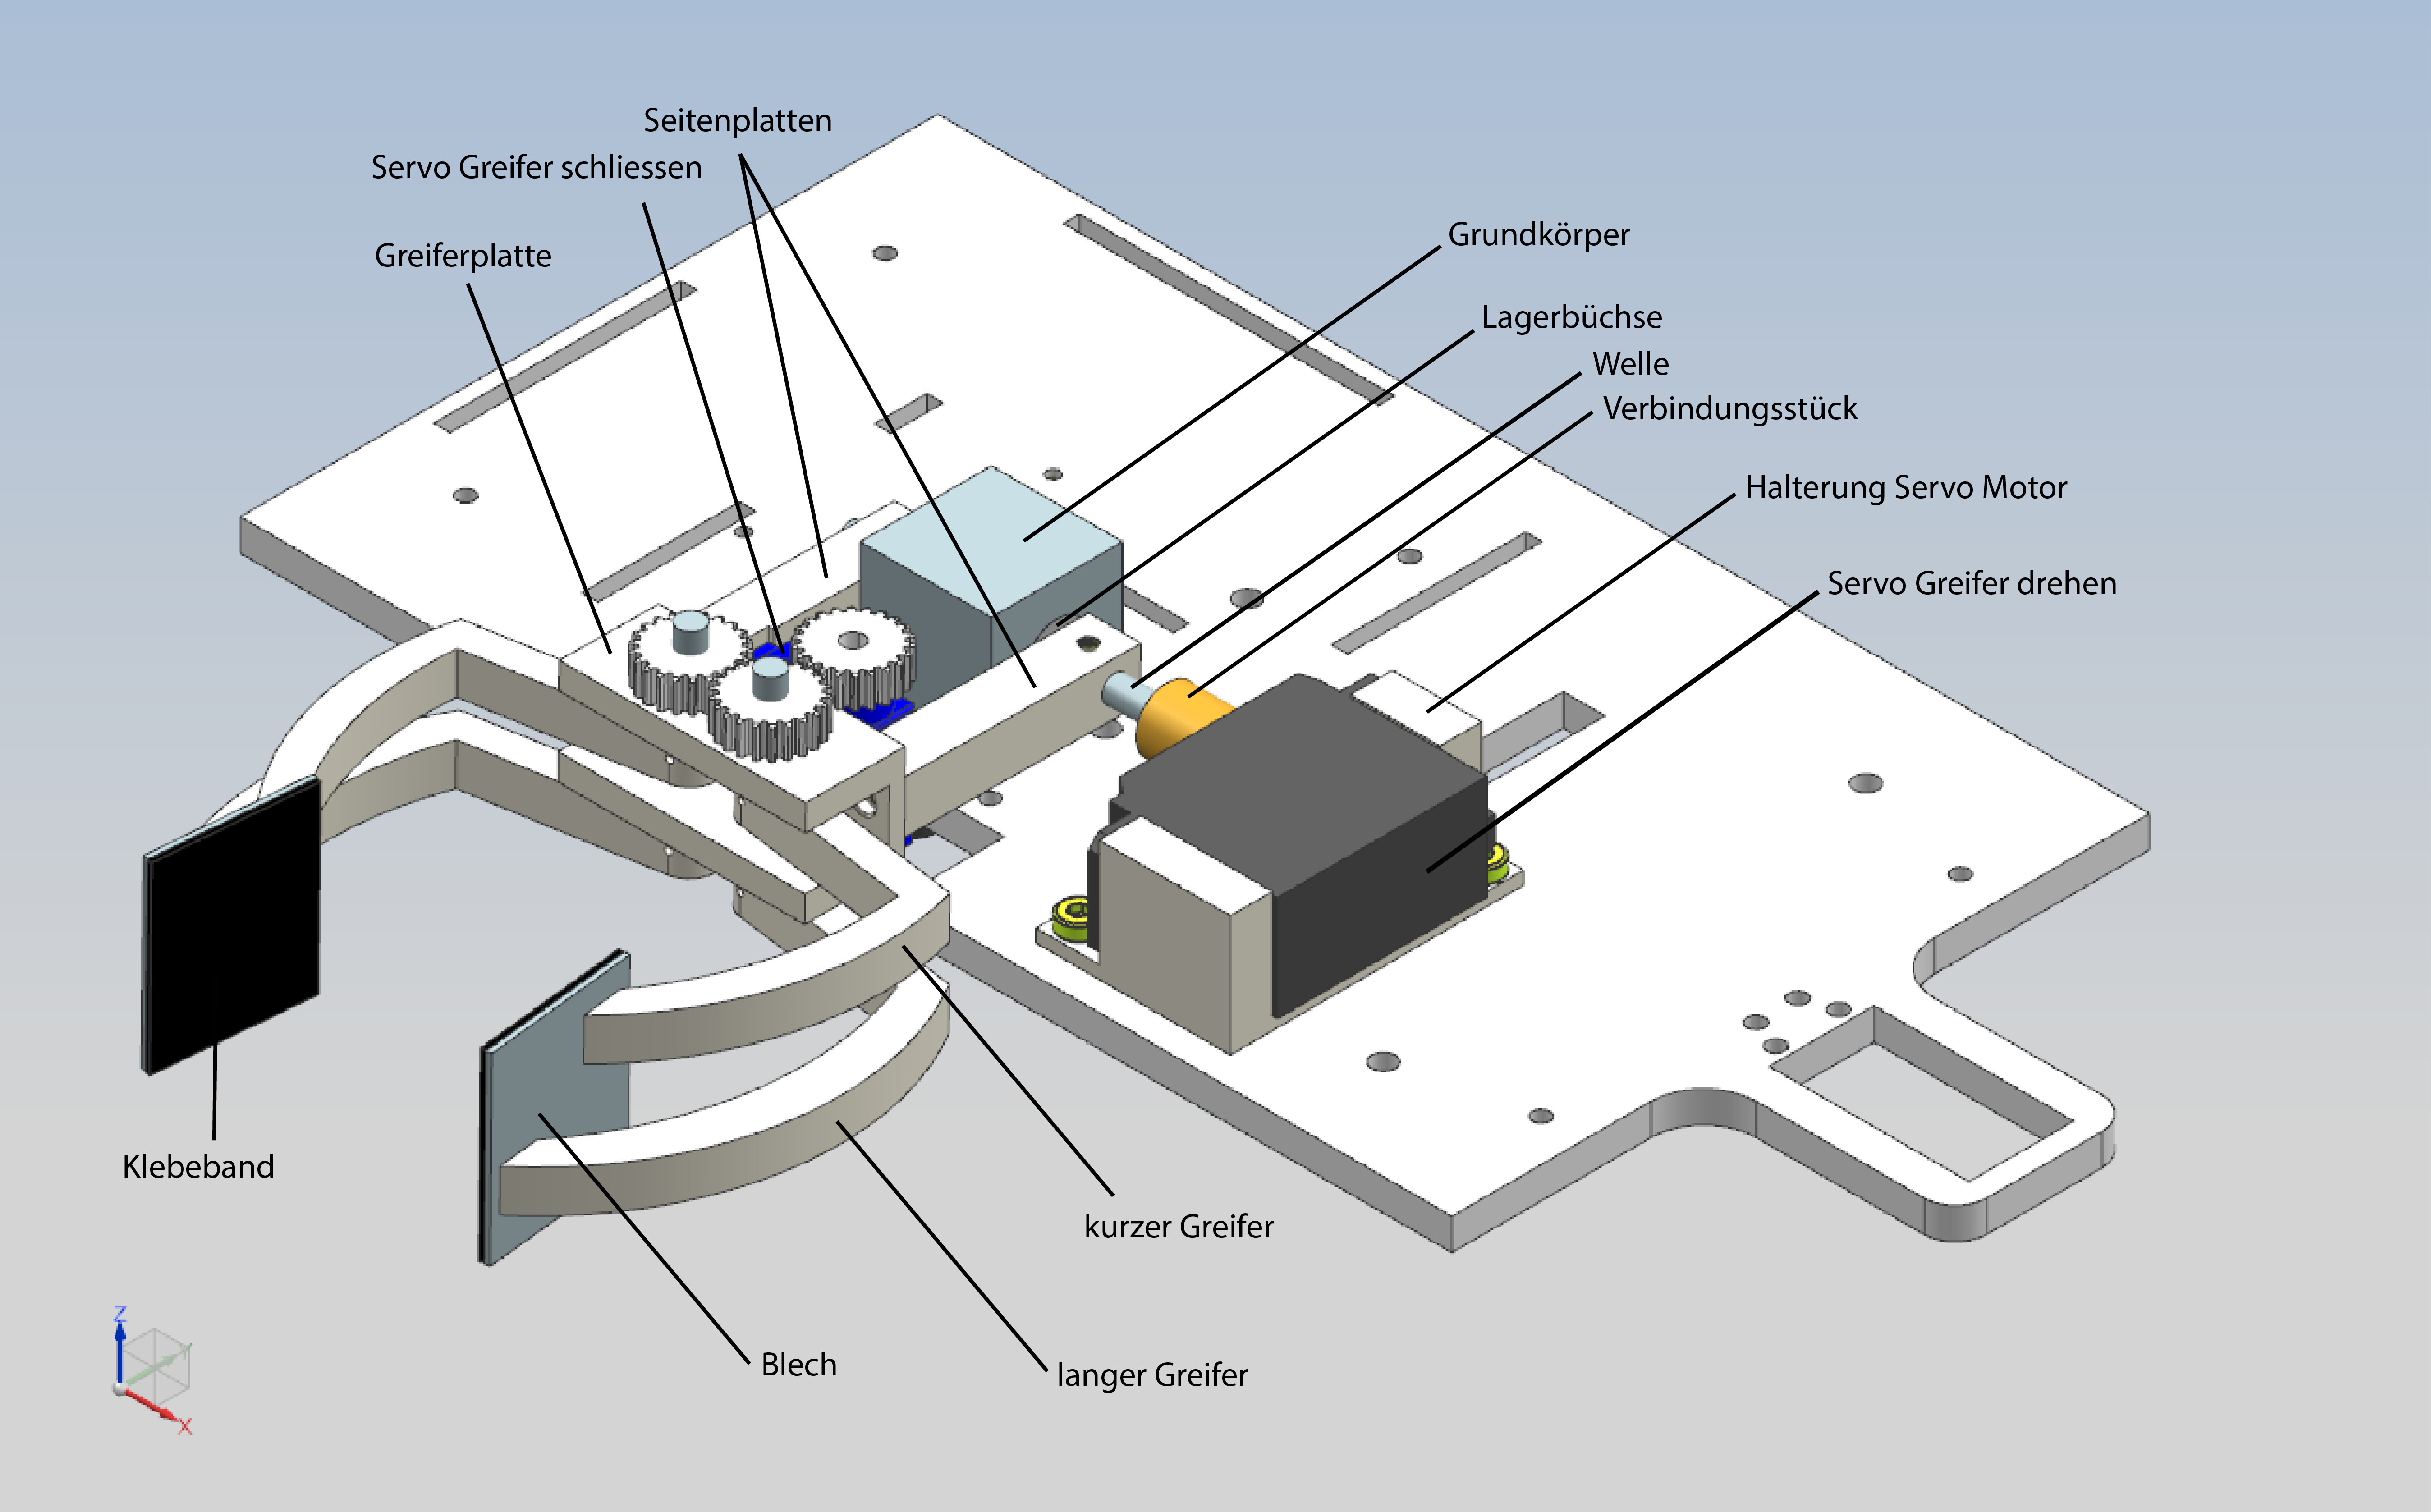
\includegraphics[width=1\textwidth]{03_Loesungskonzept/pictures/Greifer2.png}
\caption{Greifer}
\end{figure}
\textbf{Umsetzung}\\[0.2cm]
Der Grundkörper wurde von der mechanischen Werkstatt der HSLU gefertigt. Die Zeichnung ist im Anhang zu finden. In den Grundkörper wurden auf beiden Seiten Lagerbüchsen eingepresst (Einkaufsteil). Der Grundkörper ist von unten mit 2 Senkschrauben auf der Grundplatte verschraubt.
Auf der rechten Seiten wurde eine Halterung (3D Druckteil) auf die Grundplatte verschraubt. In der Halterung ist der Servo Motor für die Drehung des Greifers montiert. Dieser ist auf der Halterung verschraubt. Um die Welle und den Servo Motor zu verbinden, wird ein Verbindungsstück (gefertigt von HSLU Werkstatt) benötigt. Das Verbindungsstück wird mit zwei Gewindestiften auf dem Servo und der Welle befestigt. Auf die Welle wird die erste Seitenplatte (3D Druckteil) aufgesetzt, dann durch den Grundkörper geführt und anschliessend die zweite Seitenplatte montiert. Auf der Welle wurden 2 Flächen angebracht auf Position der Gewinde der Seitenplatten. So können die beiden Seitenplatten mit Gewindestiften auf der Welle befestigt werden. Die Greiferplatte (3D Druckteil) wurde mit Senkschrauben auf den beiden Seitenplatten verschraubt. 
Auf den beiden Seitenplatte ist der Servo Motor um den Greifer zu schliessen bzw. öffen verschraubt. Auf dem Servo ist mit einem Gewindestift ein Zahnrad (Einkaufteil) befestigt. Durch die Greiferplatte sind zwei Wellen frei drehbar gelagert. Auf diesen werden die Greifer (3D Druckteil) mit Gewindestiften wie auch die Zahnräder montiert. Die Greifer wurden möglichst parallel eingestellt und anschliessend Bleche und Klebeband befestigt.
\\
Der Greifer ist während des Fahren in obiger Position gelagert. Sobald der Container auf Höhe des Greifer ist, wird der Greifer heruntergelassen (Greifer komplett geöffnet). Die Greifer schliessen und der Greifer wird das oben gedreht. Das Schüttgut wird nun in das Behältersystem geleert. Danach wird der Greifer wieder auf die untere Stellung gefahren und der Greifer wird geöffnet, damit der Container wieder an der ursprünglichen Position steht. Zum Schluss wird der Greifer geöffnet und in Anfangsposition gedreht.\\[0.2cm]
\begin{figure}[H]
\centering
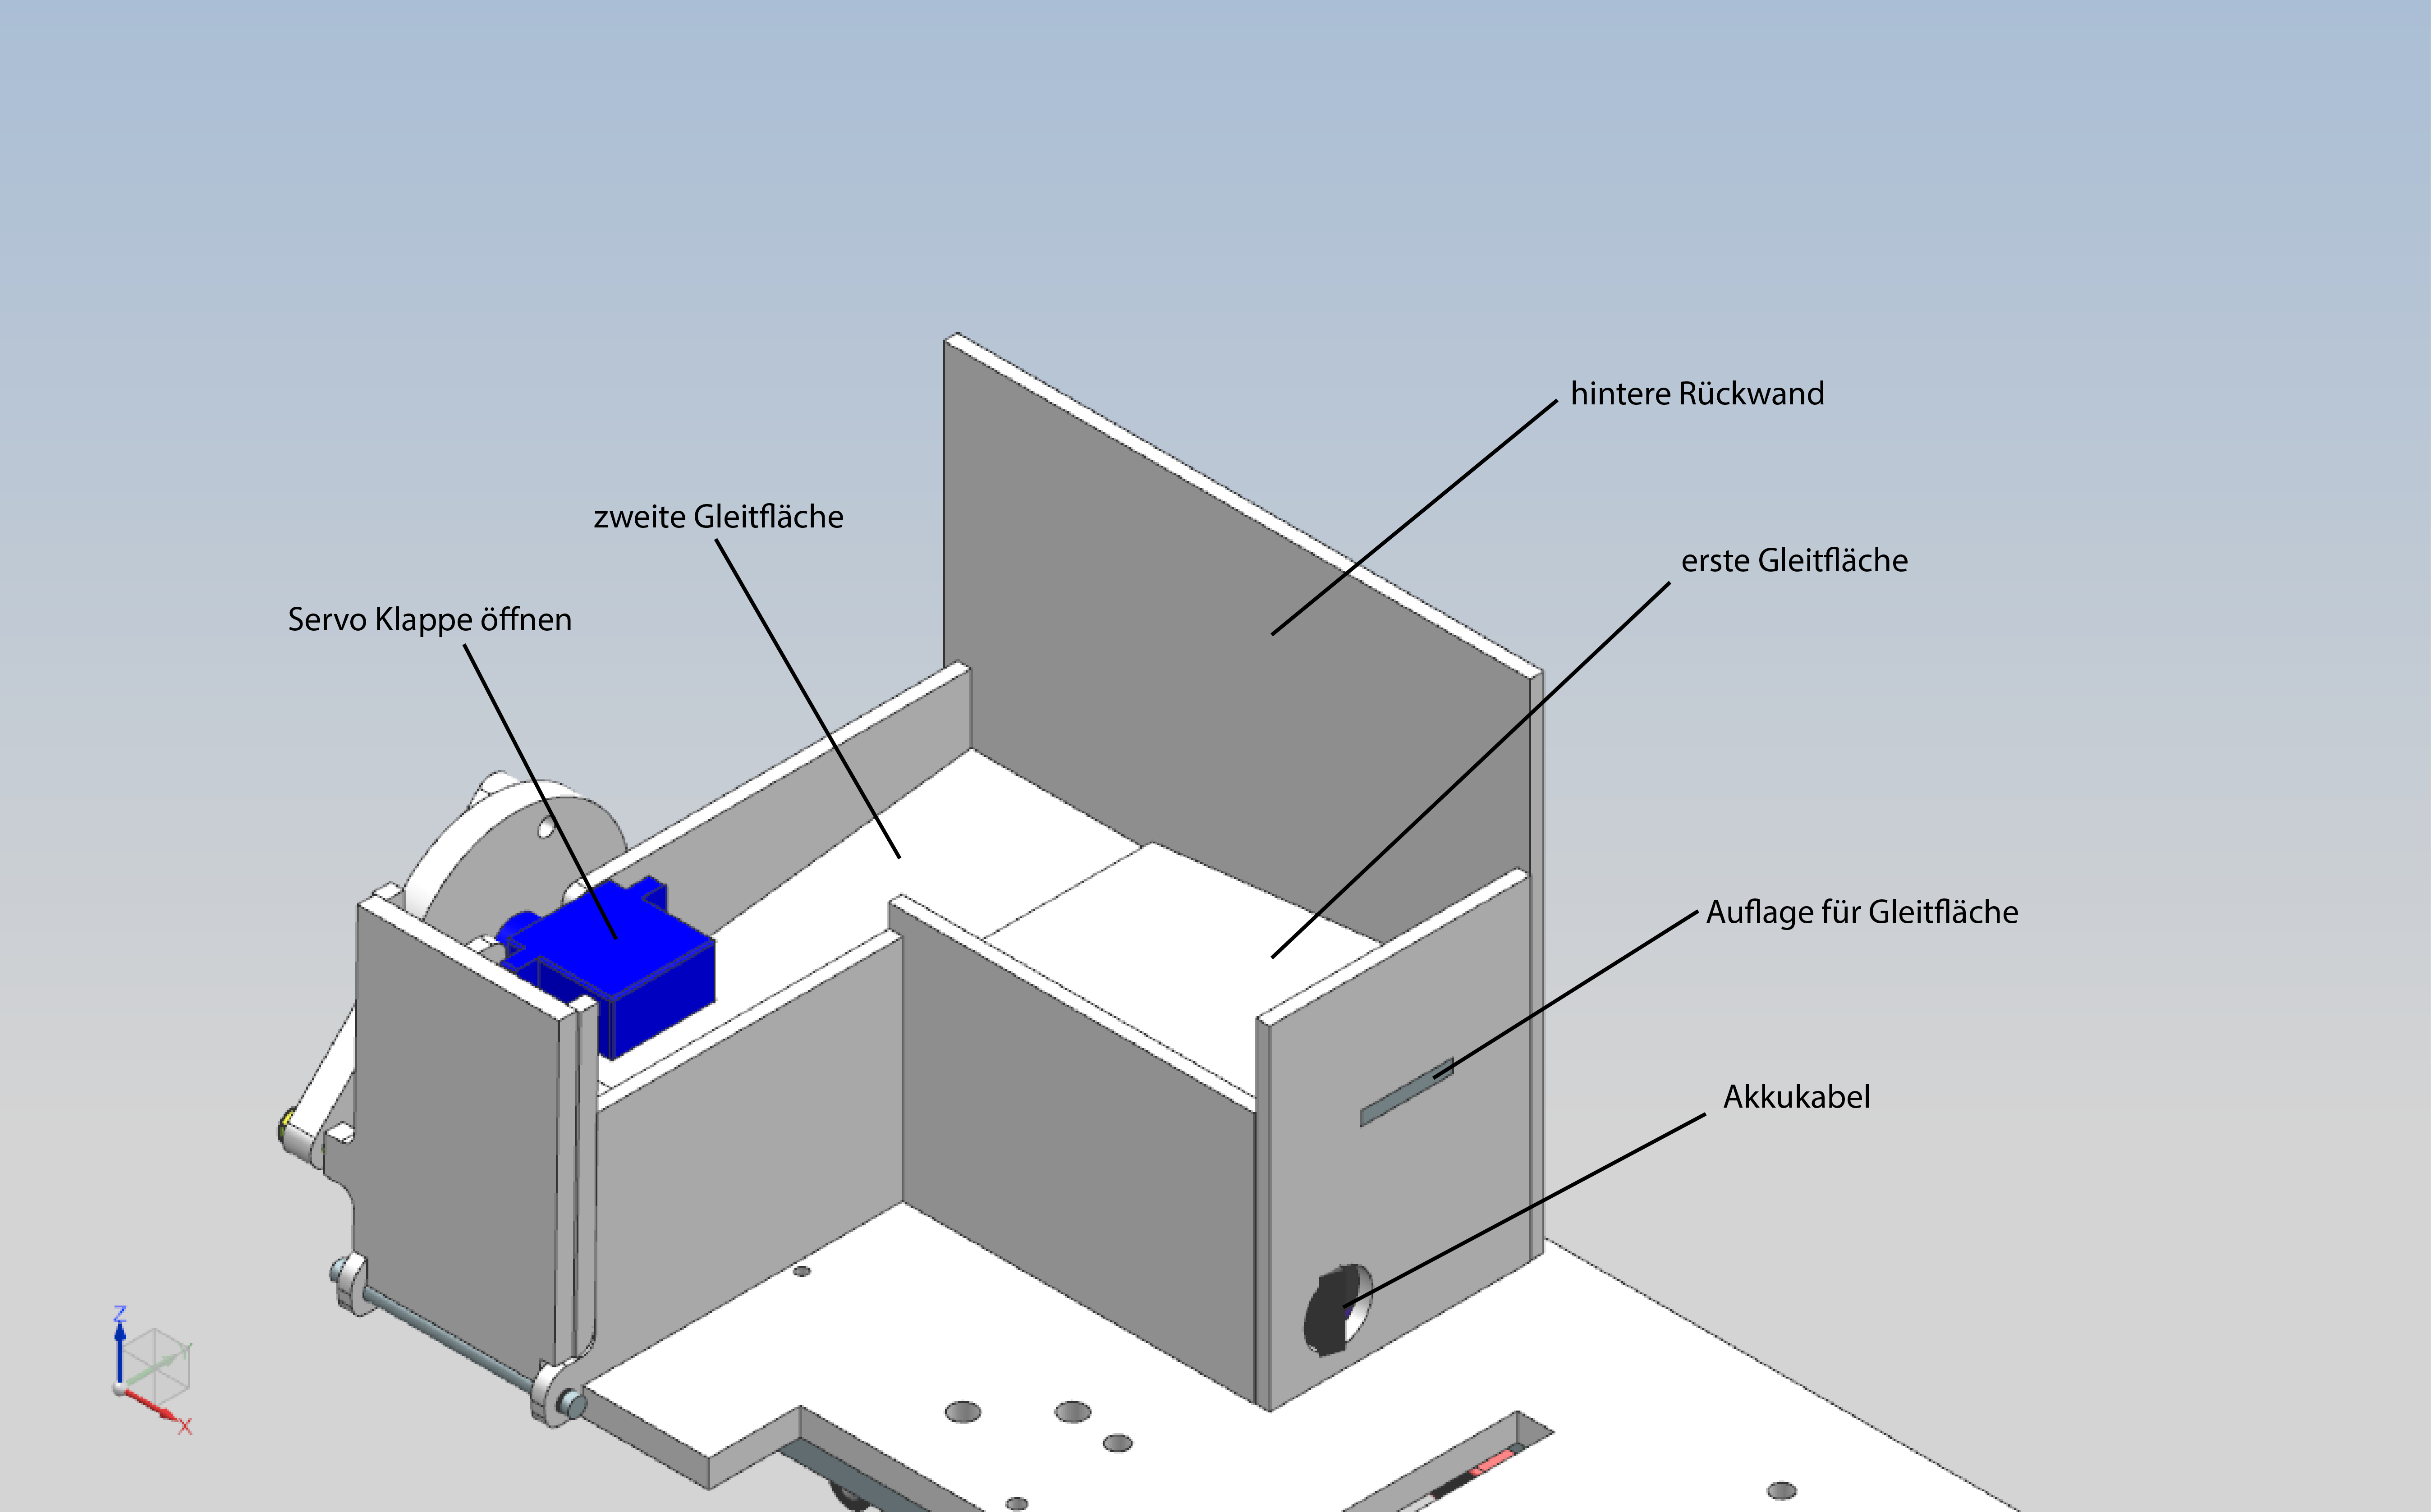
\includegraphics[width=1\textwidth]{03_Loesungskonzept/pictures/entladen11.png}
\caption{Entladebehälter}
\end{figure}
Der Container wird in den ersten Behälter entleert. Durch den schrägen Boden und die Geschwindigkeit rutscht das Schüttgut in den zweiten Behälter. Am Ende des zweiten Behälters ist eine Klappe montiert, damit die Schrauben und Muttern nicht herausfallen. Die Klappe wird durch einen Servo Motor gehalten und erst am Schluss beim Entladebehälter geöffnet.\\[0.2cm]
Die Behälterteile wurden bis auf die zweite Gleitfläche aus Acrylglas (Laserschneiden) gefertigt. Die zweite Gleitfläche ist ein 3D Druckteil.
Um die Seitenwände zu montieren wurden auf der Grundplatte Schlitze herausgelasert. Damit konnten die Behälterteile auf die Grundplatte gesteckt (0.1 mm Übermass in Länge und Breite in der Grundplatte), zudem wurden sie noch festgeklebt. Die hintere Rückwand ist absichtlich hoch, damit fliegende Schüttgutteile nicht auf die Strasse fallen können.\\[0.2cm] 
Unter dem Behältersystem befindet sich der grosse Akku. Das Kabel kann rechts durch die Behälterwand geführt werden. In der Rückwand ist ein Rechteck ausgelasert um den Akku herauszuschieben. Auf der linken Seitenwand ist auch noch ein Rechteck ausgelasert. Dort kann der Akku zum Laden entfernt werden.